%% Copernicus Publications Manuscript Preparation Template for LaTeX Submissions
%% ---------------------------------
%% This template should be used for copernicus.cls
%% The class file and some style files are bundled in the Copernicus Latex Package, which can be downloaded from the different journal webpages.
%% For further assistance please contact Copernicus Publications at: production@copernicus.org
%% https://publications.copernicus.org/for_authors/manuscript_preparation.html


%% Please use the following documentclass and journal abbreviations for discussion papers and final revised papers.

%% 2-column papers and discussion papers
\documentclass[essd, manuscript]{copernicus}

%% \usepackage commands included in the copernicus.cls:
%\usepackage[german, english]{babel}
%\usepackage{tabularx}
%\usepackage{cancel}
%\usepackage{multirow}
%\usepackage{supertabular}
%\usepackage{algorithmic}
%\usepackage{algorithm}
%\usepackage{amsthm}
%\usepackage{float}
%\usepackage{subfig}
%\usepackage{rotating}
\usepackage[ruled,vlined]{algorithm2e}

\begin{document}

\title{Decomposition of multispectral Sentinel-2 time series using neural networks for missing data imputation and compression.}


% \Author[affil]{given_name}{surname}

\Author[1]{Pablo R.}{Larraondo}
\Author[1]{Albert I. J. M.}{van Dijk}
\Author[1]{Marta}{Yebra}

\affil[1]{Fenner School of Environment and Society. Australian National University. Canberra, Australia}

%% The [] brackets identify the author with the corresponding affiliation. 1, 2, 3, etc. should be inserted.

%% If an author is deceased, please add a further affiliation and mark the respective author name(s) with a dagger, e.g. "\Author[2,$\dag$]{Anton}{Aman}" with the affiliations "\affil[2]{University of ...}" and "\affil[$\dag$]{deceased, 1 July 2019}"


\correspondence{Pablo R. Larraondo (pablo.larraondo@anu.edu.au)}

\runningtitle{TEXT}

\runningauthor{TEXT}

\received{}
\pubdiscuss{} %% only important for two-stage journals
\revised{}
\accepted{}
\published{}

%% These dates will be inserted by Copernicus Publications during the typesetting process.

\firstpage{1}

\maketitle

\begin{abstract}
TEXT
\end{abstract}

\copyrightstatement{TEXT}

\introduction  %% \introduction[modified heading if necessary]

Remote sensing provides valuable information about the Earth with an increasing level of detail in the spatial, spectral and temporal domains. Due to the size of current remote sensing collections, processing the data requires accessing large amounts of storage and compute resources, making this task difficult and expensive. In the case of studying land processes, only the reflectance component coming from the Earth's surface is used, and all other effects originating in the atmosphere, such as clouds or shadows, can be considered noise contaminating the land's signal. Changes in the land typically happen at lower temporal scales than those in the atmosphere, which suggests that the land dynamics can be described using in much lower dimensional space than the original data. This idea leads to the exploration of methodologies that exploit the inherent redundancies in the data and find efficient representations, able to capture the variability in the signal coming just from the land.

From an algebraic perspective, we can say that there exists a low-rank representation of the Earth's surface signal that is able to capture most of the variability in the original signal. Finding this low-rank representation is the objective of Principal Component Analysis (PCA). The use of PCA in remote sensing has been known for many years and it has been extensively explored in the context of noise filtering and the compression of satellite images.

One of the limitations of PCA is its inability to work with missing values. As discussed before, remote sensing images representing the land surface, are often contaminated with atmospheric signals that need to be filtered, creating gaps of missing data in the images. There are different approaches for removing missing values for applying PCA, such as, temporal aggregation of pixels, assigning fixed values to the missing data or using different forms of interpolation through space or time. Therefore, the resulting decomposition performed by the PCA would depend on the process used to estimate values for the missing data. Regardless of the quality of the method employed for removing the missing values, artificial, non-observed values are introduced in the original signal, leading to errors and biases in the resulting decomposition.

PCA calculates the principal components of a matrix as the eigenvectors of its correlation matrix. This implies that principal components constitute an orthogonal basis for reconstructing the original matrix. This orthogonality constraint ensures that the information expressed by each component is unique and independent from the others. However, from an optimisation point of view, orthogonality makes the decomposition problem to be non-convex. Removing the orthogonality constraint ensures decomposition is convex, which allows applying common optimisation techniques, such as gradient descent, to find valid decompositions of the original data. This idea of relaxing PCA constraints has been already proposed \citep{udell2014generalized} presenting a framework for generalising low-rank models.

Building upon the previous framework, this work explores how neural networks can be used to find efficient decompositions of remote sensing time series data. We evaluate the accuracy and performance of the proposed methodology comparing its results to classical PCA. Considering that the proposed methodology can naturally deal with missing values, we evaluate the quality of the resulting imputed data and compare it to other forms of pixel interpolation through time, a common approach used for applying PCA. The experiments are performed using temporal series of Sentinel-2 data over a region in Australia.


\section{Data}

The Copernicus Sentinel-2 mission \citep{drusch2012sentinel} is a constellation of two polar-orbiting satellites Sentinel-2A and Sentinel-2B launched on the 23th of June 2015 and the 7th of March 2017, respectively. These satellites are placed in the same sun-synchronous orbit and scan the Earth with a combined revisit period of 5 days and spatial resolutions that range between 10 and 60 metres. Digital Earth Australia (DEA) \citep{dhu2017digital} is a platform that contains Sentinel-2 data for Australia. DEA facilitates access and enhances quality of the data by adding further processing, such as correction for atmospheric and terrain effects. DEA data is stored using the Albers equal area projection for ensuring pixel size remains constant independent of its location.

To run the experiments in this work we extracted from DEA a 7000 km\textsuperscript{2} area around the Australian Capital Territory region comprising the years 2018 and 2019. Spectrally, we chose a subset of seven bands: three in the visible channels, two in the near infra-red and two in the short wave infrared, corresponding to bands (2, 3, 4, 8, 8a, 11, 12) in the original dataset. Bands 8a, 11 and 12 have nominal resolutions of 20 metres and were upsampled into 10 metres using nearest neighbour, to achieve a homogeneous resolution across all bands.

The data was then split using regular tiles of 4 square kilometers each, comprising the whole temporal extent. Figure \ref{dataset} shows a map of the region and the extent of each tile within a 16 by 23 grid. Using a contiguous region, as opposed to sparse isolated tiles, ensures the dataset contains a fair mix of tiles that are fully and partially filled with image data, due to random intersections with the original Sentinel-2 scenes. The objective is to consider a dataset that is manageable to carry out the experiments but that is representative of the original data. The results of this work should be easily reproduced for any other location.

\begin{figure}%
    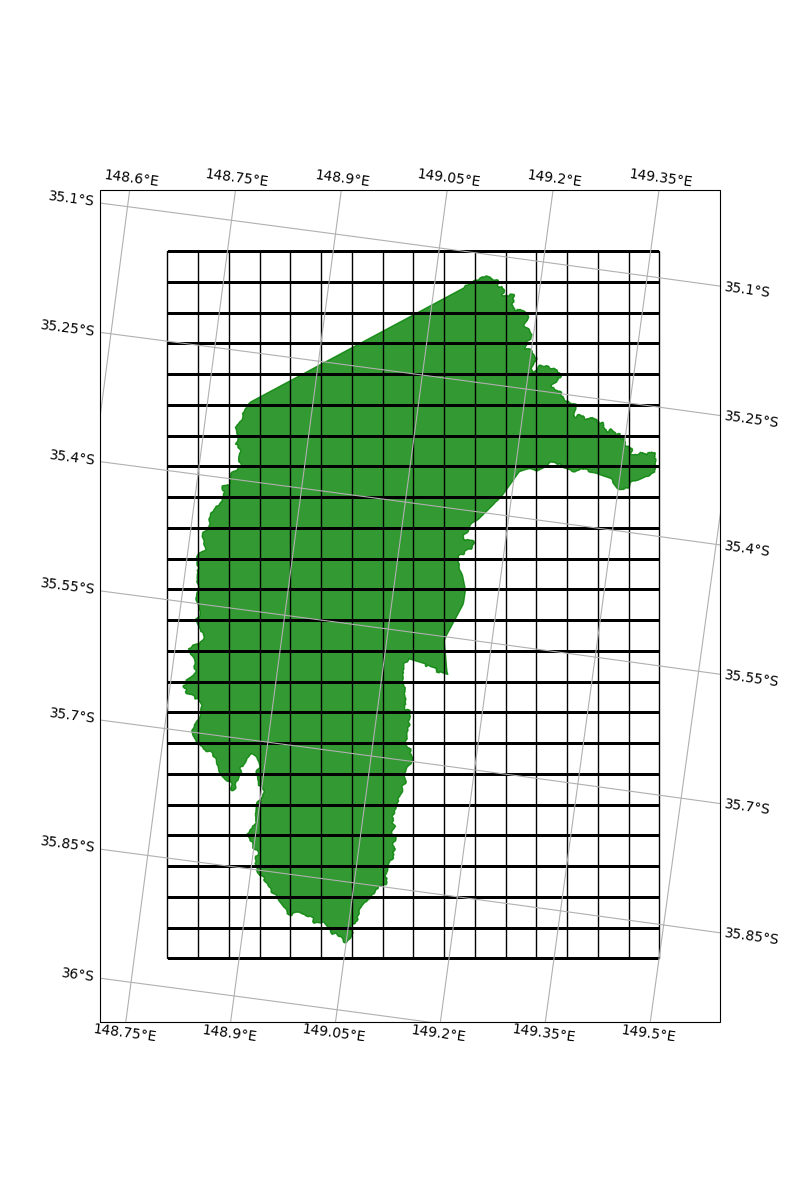
\includegraphics[width=10cm]{fig1.png}
    \caption{Region of the ACT with extents of the Sentinel 2 tiles.}%
    \label{dataset}%
\end{figure}

Each tile, as described previously, can be represented using a cube formed stacking 400 by 400 pixel images along the temporal dimension. In time, the number of images ranges between 85 and 130 depending on the position of the tile. The data was stored stacking each of the seven spectral bands in the same time dimension. Figure \ref{dataset_detail} represents the tile in the top-left corner in the dataset, with images corresponding to different dates stacked along the vertical dimension. On the left, the true colour composite is represented. On the right, the seven spectral bands are stacked together along the time dimension, as used in the experiments. 

\begin{figure}%
    {{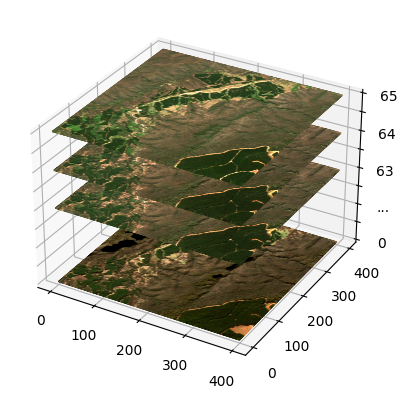
\includegraphics[width=4cm]{fig2a.png} }}%
    {{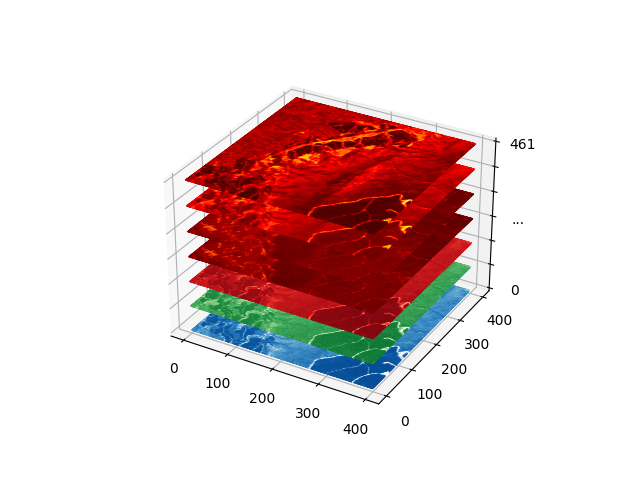
\includegraphics[width=4cm]{fig2b.png} }}%
    {{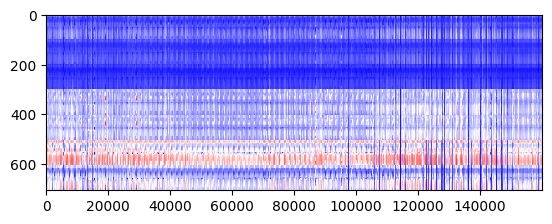
\includegraphics[width=8cm]{fig2c.png} }}%
    \caption{Tile corresponding to the top-left corner in the dataset (a) temporal stack of true colour images, (b) temporal stack of spectral images, (c) multi-spectral stack reshaped into 2-dimensional matrix}%
    \label{dataset_detail}%
\end{figure}

\subsection{Filtering clouds and shadows}
The atmosphere, standing between the satellite and the Earth's surface, modifies the spectral response coming from the ground. Clouds, haze and other atmospheric meteors affect ground measurements and can be considered as noise contaminating the signal coming from the Earth. For our experiments, we want to capture the variability coming from the ground and then, we need to remove all the other sources of variability in the data.

Several methodologies for removing clouds from Sentinel-2 images have been proposed \citep{louis2016sentinel,hagolle2017maja,qiu2019fmask}. These methodologies can be classified into single-date and multi-temporal algorithms \citep{}. For a comprehensive review and performance comparisons we refer readers to \citep{zhu2018cloud}. Multi-temporal algorithms are generally more accurate when compared to single-date ones, but have the inconvenient of being more difficult to implement and compute intensive.

In this work we propose a new simple multi-temporal methodology to detect pixels containing clouds and shadows. This methodology defines a series of dynamic thresholds using the for each pixel for determining if pixels corresponds to either clear sky, cloud or shadow categories. This methodology employs two Sentinel-2 spectral bands, blue (490 nm) and narrow nir (865 nm) and is easy to implement and efficient to run compared to other multi-temporal methods \citep{frantz2015enhancing,zhu2018automatic}.

The proposed methodology assumes a 3-dimensional array of images stacked along time. 

Atmospheric processes normally have a much higher temporal variability than the ones occurring on the Earth's surface. Temporal based methods exploit this difference in the variability to detect outliers that can be attributed to atmospheric processes. Temporal based methods  


\section{Methodology}

Principal Component Analysis (PCA) of a matrix $M$ is typically computed via the singular value decomposition (SVD). The Eckart-Young theorem \citep{eckart1936approximation}, proves that this decomposition, truncated to the first $n$ factors, is the best rank-n approximation in the least squares sense, amongst all possible decompositions of $M$. Although PCA achieves the best factorisation of $M$, its solution is not unique and other methods can be employed to find alternative decompositions with the same error. 

From an optimisation point of view, this matrix factorisation problem can be formulated as:

$$
\arg\:\min_{AB} \mathbf{MSE}(M-AB)
$$

Where $\mathbf{MSE}$ stands for the mean square error and $A$ and $B$ are the factor matrices to optimise. The objective of this optimisation problem is to find the best $A$ and $B$ matrices whose product gives the best approximation of $M$.

In this work, we employ neural networks to solve this problem using gradient descent optimisation. The model can be expressed using a two layers neural network where each layer represents one factor matrix. The neural network then is trained to minimise the distance between the original matrix $M$ and the product of the two layers corresponding to factors $A$ and $B$. This network does not make use of non-linear activations resulting in a linear model.


As described in the previous section, we consider $M$ to be the matrix containing temporal series of satellite images, represented in Figure \ref{dataset_detail} c). We assume that the dynamics of the landscape, expressed through the evolution in time of the different spectral bands, can be expressed by a matrix $M'$, that has significantly lower rank than the original matrix. This rank can be determined truncating the size of the decomposed matrices at a certain level, or in terms of PCA decomposition, by limiting the number of the factored principal components. As the number components is increased, the error in the factorisation is reduced, getting to zero when the number of components equals the rows of $M$, which corresponds to the size of the temporal dimension. Figure \ref{explained_variance_evolution} represents the evolution of the explained variance in the recovered matrix $M'$ as the number of components is increased. To perform the experiments in this work, we fixed the number of components to 12, which gives a good compromise between the quality of the recovered signal and the compression ratio. 


Figure \ref{factorisation} represents the reconstruction of the unbiased satellite observation matrix, $M$, as the product of two matrices, $A$ and $B$. Matrix $M$ in this case contains 138 rows and 160000 columns, corresponding to the temporal dimension and number of pixels (400x400) respectively. In this representation, the number of components is truncated to 12. Matrix $B$ is then a matrix with size (12, 160000) corresponding to 12 principal components and the 400x400 spatial shape of the orignal tiles. Matrix $A$ contains the coefficients that multiply each of the principal components to recreate the temporal entries in the original matrix $M$. The number of columns of $A$ is the same as the rows of $B$, and this number determines the truncation performed to the reconstruction. This number sets therefore a trade-off between the achieved accuracy in the reconstruction and the compression ratio of the original matrix $M$. In this case, considering the total size of the matrices on each side of the equality, we get that the factors are $(138 \cdot 160000) / ((138 \cdot 12) + (12 \cdot 160000)) = 84 $ times smaller when compared to $M$. 

\begin{figure}%
    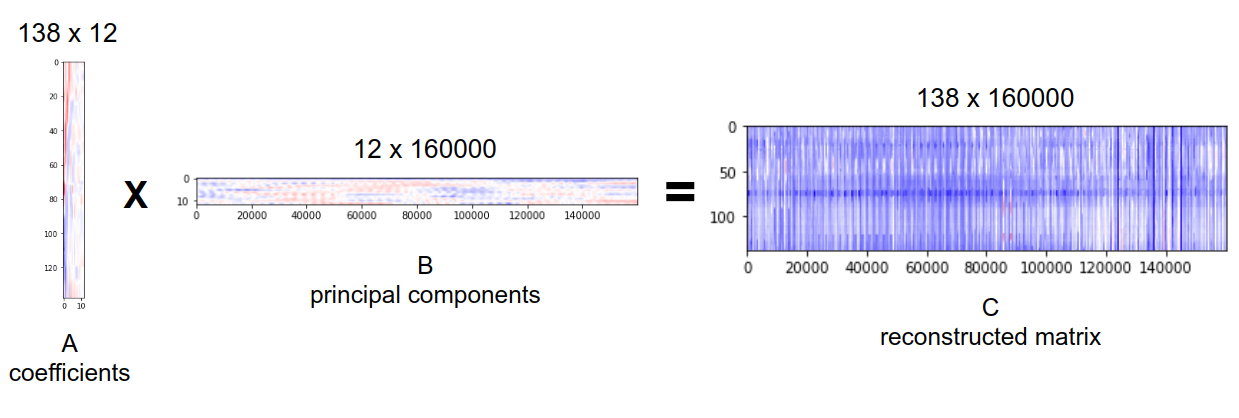
\includegraphics[width=10cm]{fig3.png}
	\caption{Reconstruction of the matrix of observations as the product of two factorised matrices, known as the matrix of coefficients (left) and principal components (right) in the case of PCA.}%
    \label{factorisation}%
\end{figure}

The proposed methodology uses NNs to compute the factor matrices $A$ and $B$. Nevertheless, the reconstruction process presented in Figure \ref{factorisation} and size of the matrices remains the same as in the case of PCA. In PCA, we commonly refer to $A$ as the coefficients matrix and $B$ as the principal components matrix. Although the NN methodology generates different factorisations to PCA, we intentionally use the same terminology to refer to these factor matrices for stablishing a link between both methodologies and improving clarity.

\begin{figure}%
    {{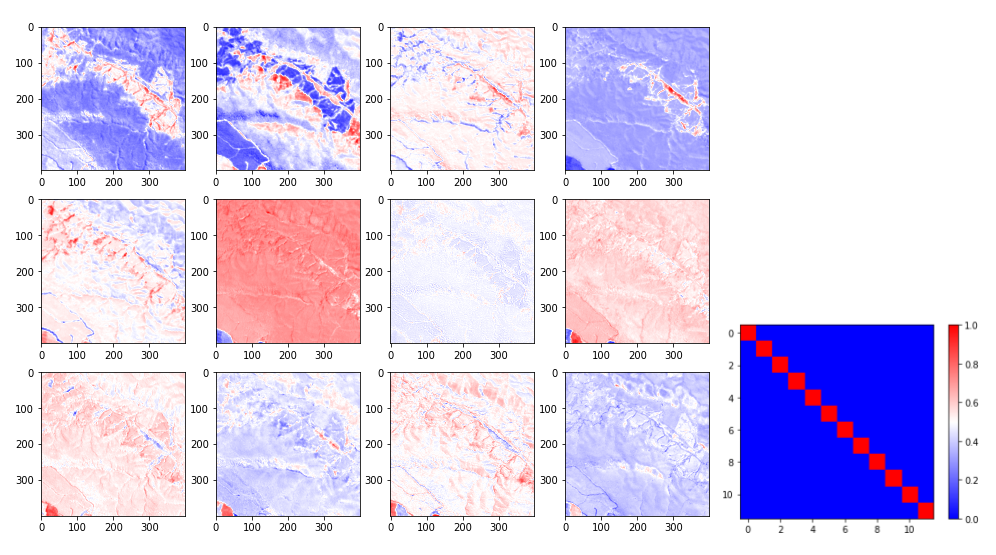
\includegraphics[width=8cm]{fig4a.png} }}%
    {{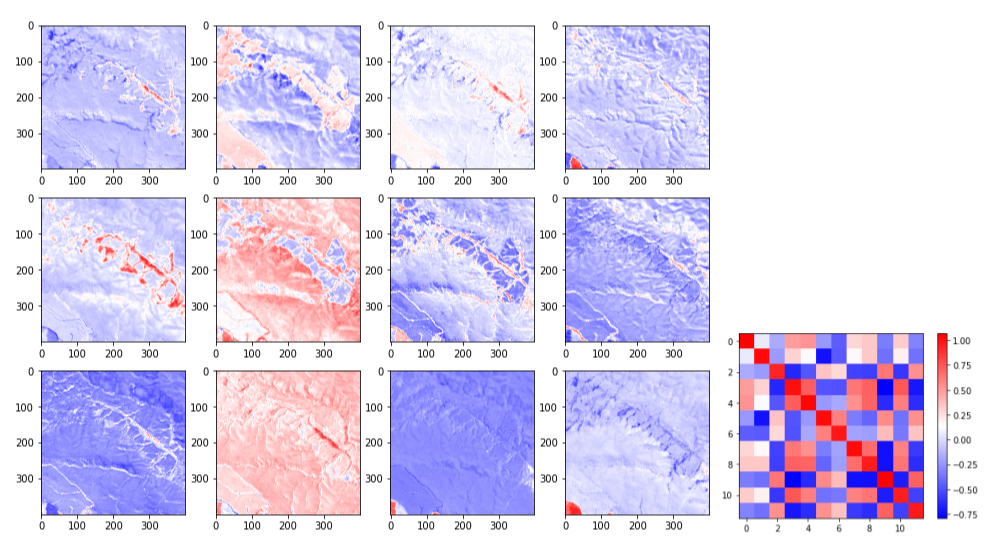
\includegraphics[width=8cm]{fig4b.png} }}%
	\caption{Representation of the 12 principal components matrix in Figure \ref{factorisation} as calculated by PCA (left) and the NN (right). Each component has been reshaped into the original 400x400 size of the original tiles.}%
    \label{pcs}%
\end{figure}

Figure \ref{pcs} represents the 12 principal components in matrix $B$ computed using PCA (left) and NN (right) reshaped into the original 400x400 size of the stack of images. The plots on the lower right show the product $B^TB$, which represents the inner products between each component. In the case of PCA, $B^TB$, shows entries equal to one along the main diagonal and zero everywhere else. This confirms that principal components resulting from PCA form an orthonormal basis. On the right, the $B^TB$ resulting from the NN factorisation, has heterogeneous values across the matrix, which means that the computed components are not orthogonal. Another difference between both methodologies is that the principal components computed with PCA are ordered by importance at explaining the variance in the original signal (from top-left to the bottom-right) but not such ordering exists in the case of NN (this can be verified looking at the values of the coefficients matrix in each case). We note that as opposed to PCA, the decomposition achieved with the NN method is not unique and varies between runs. The order of the components (columns of $B$) and also the magnitude of the matrices elements can vary and still generate the same product.

In the next section we perform a series of experiments to assess the ability of the NN methodology to impute missing entries compared to temporal interpolation. These results are then compared with temporally interpolated PCA. To ensure a fair comparison between methodologies, we randomly masked known portions in the image stack and assessed the imputed and interpolated values with the original unmasked values.


\section{Experimental Results and Discussion}


In order to compare the accuracy of the imputed missing data of our method we perform an experiment to 

A mask with 
The stack of images containing gaps of missing values is further processed data containing 
To carry out this experiment we generate three version of the same dataset: (1) The 
There are therefore three versions of the tile 
The training process of the 
by the imputation 

\begin{figure}%
    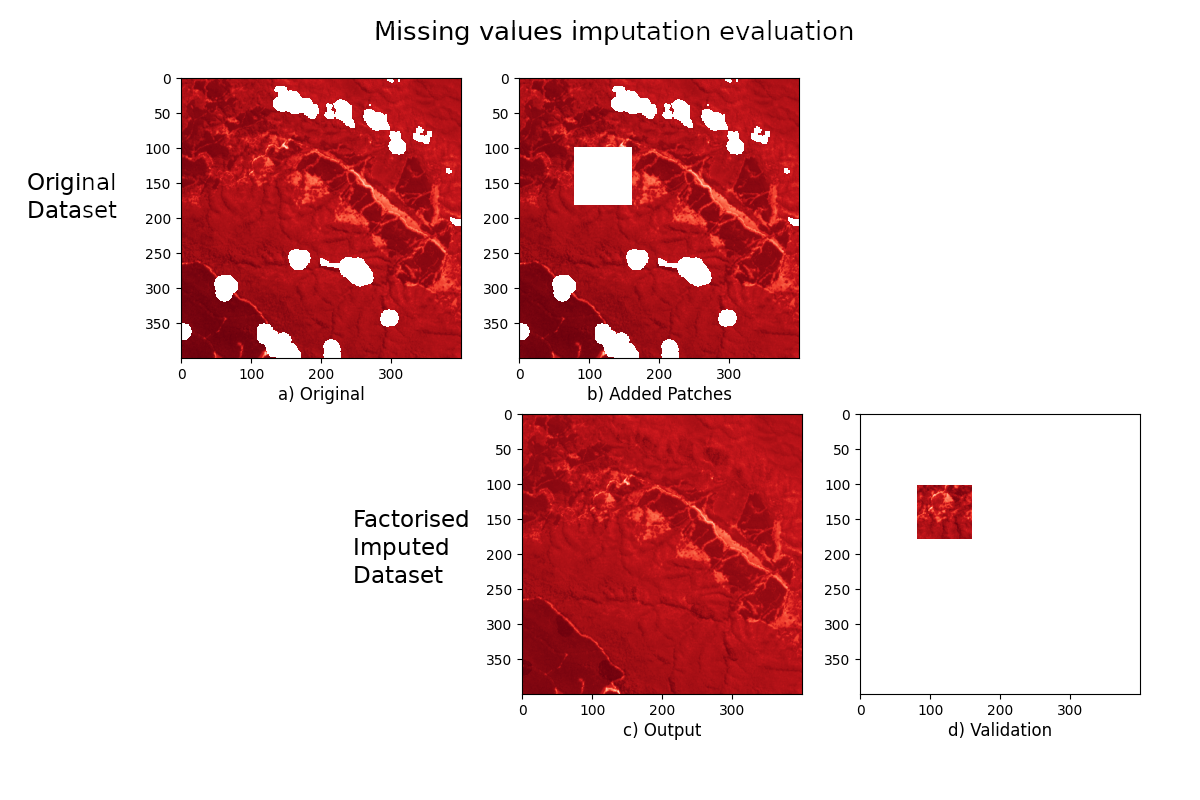
\includegraphics[width=10cm]{fig5.png}
    \caption{Masking process for comparing missing data imputation accuracy.}%
    \label{dataset_versions}%
\end{figure}

Figure \ref{dataset_versions} represents 


\conclusions  %% \conclusions[modified heading if necessary]
In this paper, we evaluated the application of NNs to decompose remote sensing data in the presence of missing values as an alternative to other interpolation methods. The methodology was evaluated to Sentinel-2 time series data for the Australian Capital Territory region. The NN-based methodology achieved better compression ratios and accuracy at interpolating missing values when compared to PCA. We demonstrate that relaxing the orthogonality constraints of PCA improves compression for time series of satellite multispectral data.

Additional studies are planned to evaluate the effect of non-linearities and convolution operations in the network. Another avenue for exploration is the introduction of constraints that lead to sparsity to enhance compression and improve interpretability of the results. 

%% The following commands are for the statements about the availability of data sets and/or software code corresponding to the manuscript.
%% It is strongly recommended to make use of these sections in case data sets and/or software code have been part of your research the article is based on.

%\codeavailability{TEXT} %% use this section when having only software code available


%\dataavailability{TEXT} %% use this section when having only data sets available


\codedataavailability{} 
%% use this section when having data sets and software code available
The code used to process the data and run the experiments in this paper is publicly available at: \\
\href{https://github.com/prl900/unet_him8_gpm}{https://github.com/prl900/unet\_him8\_gpm}. \\
Sentinel-2 Surface Reflectance NBART data used in the experiments comes from Geoscience Australia's Digital Earth Platform \href{https://cmi.ga.gov.au/data-products/dea/190/dea-surface-reflectance-nbart-sentinel-2-msi}{https://cmi.ga.gov.au/data-products/dea/190/dea-surface-reflectance-nbart-sentinel-2-msi}. 

%\sampleavailability{TEXT} %% use this section when having geoscientific samples available

%\videosupplement{} %% use this section when having video supplements available

\appendix
\section{Cloud \& shadow masking algorithm} %% Appendix A

The cloud and shadow filtering process followed in this work can be described using two steps. In a first step, bright pixels are removed using the blue channel and then two rolling median through time are calculated for the blue and narrow near-infrared channels. Remaining missing data are filled using nearest neighbour interpolation through time. The result of this step are two arrays of the same dimensions as the initial ones where pixels with high reflectance values on the blue channel have been removed and the values of the pixels are smooth in time using a temporal median filter. The purpose of this step is to have a clean stack of images that captures long term trends in the signal to be used as reference in the next step.

Useful??? Changes in reflectance values or local textures that are separable from changes caused by other factors such as differences in atmospheric conditions, illumination and viewing angles, and soil moistures \citep{deng2008pca}.

\begin{algorithm}[H]
\SetAlgoLined
 \Comment{\#1. Load Sentinel-2 data from spatial and temporal extents}\\
 blue = load(ds:sentinel2, band:blue, x:[xstart,xend], y:[ystart,yend],time:[tstart,tend])\\
 nnir = load(ds:sentinel2, band:narrow\_nir, x:[xstart,xend], y:[ystart,yend],time:[tstart,tend])\\
 \\
 \Comment{\#2. Assign pixels with blue reflectances exceeding lower quartile value by more than 10\% to NaN.}\\
 blue[(blue - blue.percentile(0.25)) $>$ 0.1] = NaN\\
 nnir[(blue - blue.percentile(0.25)) $>$ 0.1] = NaN\\
 \\
 \Comment{\#3. Entirely wipe images with more than 66\% missing pixels}\\
 blue[(blue.count\_nan(axis=1,2) $>$ width*hight*0.66] = NaN\\
 nnir[(nnir.count\_nan(axis=1,2) $>$ width*hight*0.66] = NaN\\
 \\
 \Comment{\#4. Calculate rolling median along time dimension and interpolate missing values}\\
 blue\_median = blue.rolling\_median(window\_size=7).interpolate(method=nearest)\\
 nnir\_median = nnir.rolling\_median(window\_size=7).interpolate(method=nearest)\\
 \caption{Step 1: rolling median calculation.}
\end{algorithm}

The second step uses these rolling median stacks to detect anomalies in the original stacks. 

\begin{algorithm}[H]
\SetAlgoLined
 \Comment{\#1. Load Sentinel-2 data from spatial and temporal extents}\\
 blue = load(ds:sentinel2, band:blue, x:[xstart,xend], y:[ystart,yend],time:[tstart,tend])\\
 nnir = load(ds:sentinel2, band:narrow\_nir, x:[xstart,xend], y:[ystart,yend],time:[tstart,tend])\\
 
 \Comment{\#2. Calculate rolling medians using previous algorithm}\\
 blue\_median = step1(blue)\\
 nnir\_median = step1(nnir)\\
 
 \Comment{\#3. Calculate mask using deviations from the rolling median values}\\
 blue\_mask = (blue - blue\_median) $>$ 0.01 + blue\_median/2\\
 nnir\_mask = (nnir - nnir\_median) $<$ -0.06 + nnir\_median/16\\
 mask = blue\_mask $\parallel$ nnir\_mask\\
 \\
 \Comment{\#4. Remove small clusters and dilate remaining ones}\\
 mask = remove\_small\_objects(mask, min\_size=9)\\
 mask = dilate(mask, disk=9)\\
 \caption{Step 2: Mask calculation using deviations from the blue and narrow nir rolling means.}
\end{algorithm}

These algorithms have been specified in pseudo-code using a notation similar to Python's Numpy and Xarray libraries. We refer readers to \href{https://github.com/prl900/unet_him8_gpm}{https://github.com/prl900/unet\_him8\_gpm} for a working implementation of this algorithm.

%\subsection{}     %% Appendix A1, A2, etc.


\noappendix       %% use this to mark the end of the appendix section

%% Regarding figures and tables in appendices, the following two options are possible depending on your general handling of figures and tables in the manuscript environment:

%% Option 1: If you sorted all figures and tables into the sections of the text, please also sort the appendix figures and appendix tables into the respective appendix sections.
%% They will be correctly named automatically.

%% Option 2: If you put all figures after the reference list, please insert appendix tables and figures after the normal tables and figures.
%% To rename them correctly to A1, A2, etc., please add the following commands in front of them:

\appendixfigures  %% needs to be added in front of appendix figures

\appendixtables   %% needs to be added in front of appendix tables

%% Please add \clearpage between each table and/or figure. Further guidelines on figures and tables can be found below.



%\authorcontribution{TEXT} %% this section is mandatory

%\competinginterests{TEXT} %% this section is mandatory even if you declare that no competing interests are present

%\disclaimer{TEXT} %% optional section

\begin{acknowledgements}
Re-emergence or ANU-WALD bushfire centre? Ask Marta
We gratefully acknowledge the support of NVIDIA Corporation with the donation of the Titan Xp GPU used in this research.
\end{acknowledgements}




%% REFERENCES

%% The reference list is compiled as follows:

%%\begin{thebibliography}{}

%%\bibitem[AUTHOR(YEAR)]{LABEL1}
%%REFERENCE 1

%%\bibitem[AUTHOR(YEAR)]{LABEL2}
%%REFERENCE 2

%%\end{thebibliography}

%% Since the Copernicus LaTeX package includes the BibTeX style file copernicus.bst,
%% authors experienced with BibTeX only have to include the following two lines:
%%
\bibliographystyle{copernicus}
\bibliography{refs.bib}
%%
%% URLs and DOIs can be entered in your BibTeX file as:
%%
%% URL = {http://www.xyz.org/~jones/idx_g.htm}
%% DOI = {10.5194/xyz}


%% LITERATURE CITATIONS
%%
%% command                        & example result
%% \citet{jones90}|               & Jones et al. (1990)
%% \citep{jones90}|               & (Jones et al., 1990)
%% \citep{jones90,jones93}|       & (Jones et al., 1990, 1993)
%% \citep[p.~32]{jones90}|        & (Jones et al., 1990, p.~32)
%% \citep[e.g.,][]{jones90}|      & (e.g., Jones et al., 1990)
%% \citep[e.g.,][p.~32]{jones90}| & (e.g., Jones et al., 1990, p.~32)
%% \citeauthor{jones90}|          & Jones et al.
%% \citeyear{jones90}|            & 1990



%% FIGURES

%% When figures and tables are placed at the end of the MS (article in one-column style), please add \clearpage
%% between bibliography and first table and/or figure as well as between each table and/or figure.


%% ONE-COLUMN FIGURES

%%f
%\begin{figure}[t]
%\includegraphics[width=8.3cm]{FILE NAME}
%\caption{TEXT}
%\end{figure}
%
%%% TWO-COLUMN FIGURES
%
%%f
%\begin{figure*}[t]
%\includegraphics[width=12cm]{FILE NAME}
%\caption{TEXT}
%\end{figure*}
%
%
%%% TABLES
%%%
%%% The different columns must be seperated with a & command and should
%%% end with \\ to identify the column brake.
%
%%% ONE-COLUMN TABLE
%
%%t
%\begin{table}[t]
%\caption{TEXT}
%\begin{tabular}{column = lcr}
%\tophline
%
%\middlehline
%
%\bottomhline
%\end{tabular}
%\belowtable{} % Table Footnotes
%\end{table}
%
%%% TWO-COLUMN TABLE
%
%%t
%\begin{table*}[t]
%\caption{TEXT}
%\begin{tabular}{column = lcr}
%\tophline
%
%\middlehline
%
%\bottomhline
%\end{tabular}
%\belowtable{} % Table Footnotes
%\end{table*}
%
%%% LANDSCAPE TABLE
%
%%t
%\begin{sidewaystable*}[t]
%\caption{TEXT}
%\begin{tabular}{column = lcr}
%\tophline
%
%\middlehline
%
%\bottomhline
%\end{tabular}
%\belowtable{} % Table Footnotes
%\end{sidewaystable*}
%
%
%%% MATHEMATICAL EXPRESSIONS
%
%%% All papers typeset by Copernicus Publications follow the math typesetting regulations
%%% given by the IUPAC Green Book (IUPAC: Quantities, Units and Symbols in Physical Chemistry,
%%% 2nd Edn., Blackwell Science, available at: http://old.iupac.org/publications/books/gbook/green_book_2ed.pdf, 1993).
%%%
%%% Physical quantities/variables are typeset in italic font (t for time, T for Temperature)
%%% Indices which are not defined are typeset in italic font (x, y, z, a, b, c)
%%% Items/objects which are defined are typeset in roman font (Car A, Car B)
%%% Descriptions/specifications which are defined by itself are typeset in roman font (abs, rel, ref, tot, net, ice)
%%% Abbreviations from 2 letters are typeset in roman font (RH, LAI)
%%% Vectors are identified in bold italic font using \vec{x}
%%% Matrices are identified in bold roman font
%%% Multiplication signs are typeset using the LaTeX commands \times (for vector products, grids, and exponential notations) or \cdot
%%% The character * should not be applied as mutliplication sign
%
%
%%% EQUATIONS
%
%%% Single-row equation
%
%\begin{equation}
%
%\end{equation}
%
%%% Multiline equation
%
%\begin{align}
%& 3 + 5 = 8\\
%& 3 + 5 = 8\\
%& 3 + 5 = 8
%\end{align}
%
%
%%% MATRICES
%
%\begin{matrix}
%x & y & z\\
%x & y & z\\
%x & y & z\\
%\end{matrix}
%
%
%%% ALGORITHM
%
%\begin{algorithm}
%\caption{...}
%\label{a1}
%\begin{algorithmic}
%...
%\end{algorithmic}
%\end{algorithm}
%
%
%%% CHEMICAL FORMULAS AND REACTIONS
%
%%% For formulas embedded in the text, please use \chem{}
%
%%% The reaction environment creates labels including the letter R, i.e. (R1), (R2), etc.
%
%\begin{reaction}
%%% \rightarrow should be used for normal (one-way) chemical reactions
%%% \rightleftharpoons should be used for equilibria
%%% \leftrightarrow should be used for resonance structures
%\end{reaction}
%
%
%%% PHYSICAL UNITS
%%%
%%% Please use \unit{} and apply the exponential notation


\end{document}
